\documentclass{article}
\usepackage[bottom=2.54cm, right=2.54cm, left=2.54cm, top=2.54cm]{geometry}
\usepackage{amsmath}
\usepackage{amssymb}
\usepackage{amsthm}
\usepackage{enumitem}
\usepackage{exercise} % Exercises Style
\usepackage{graphicx}
\usepackage{caption}
\usepackage{environ}
\usepackage{tabularx}  % Add this to your preamble if not already there
\usepackage{booktabs}



% Enable Code
\usepackage{minted}
\let \extra T

\newcommand{\vect}[1]{\boldsymbol{#1}}
\DeclareMathOperator{\Tr}{Tr}
\DeclareMathOperator{\Cov}{Cov}
\DeclareMathOperator{\Var}{Var}
\DeclareMathOperator{\E}{E}

\usepackage{fancyhdr}
\newenvironment{solution}
  {\renewcommand\qedsymbol{$\blacksquare$}\begin{proof}[Solution]$ $}
  {\end{proof}}

\title{Report on Autoencoder and Gaussian Mixture Model}
\author{Group 2}
\begin{document}

\pagestyle{fancy}
\fancyhf{}%
\fancyhead[L]{\textbf{ DS5230 \ Group Assignment 2 }}
\fancyhead[R]{\textbf{Group 2}}
\fancyfoot[C]{\thepage}%
\maketitle


\section*{Introduction}
In this assignment, we explore the practical application of autoencoder and guassian mixture clustering on the arxiv journal embeddings we generated for the group project. We visualized the results of the autoencoder and guassian mixture model using t-SNE and evaluate their clustering performance. We've found that the autoencoder is able to learn a compact representation of the data. However, non-neural network dimensional reduction method like U-MAP outperforms it in the context of our dataset.

\section*{The Arxive Dataset and Embeddings Generation}
We obtained the dataset by fetching papers based on multiple curated lists of influential AI/ML papers and perform a manual categorization of the papars. The original categorization are the followings: classic machine learning, optimization, neural network foundation, computer vision, reinforcement learning, representation theory, natural language processing, generative model.   However, the number of papers in each general category is not balanced, categories like computer vision and natural language processing have a lot more papers than optimization and reinforcement learning. To fix this, we merged a few categories together. The final categories have the following counts: machine learning general (89), NLP (56), Computer Vision Pattern Recognition (53), Computer Vision Generative Model(53), Recurrent Neural Network (36), Audio (25), Reinforcement Learning (18).

We use pre-trained Sentence-BERT models to generate the embeddings. Based on the MTEB benchmarks \cite{enevoldsen2025mmtebmassivemultilingualtext}, we selected the 2 of the top models that score high metrics and have less than 1B parameters. The models are: gte-multilingual-base\cite{zhang2024mgte} and jasper-vision-language \cite{zhang2025jasperstelladistillationsota} and the embedding dimension for each model is 768 and 1024 respectively. We've evaluated the performance of the embedding models in our group project and found that the jasper-vision-language slightly outperforms the gte-multilingual-base model in terms of clustering performance, measured with calinski-harabasz index, davis-bouldin index and visual inspection of clusters. Therefore, we will use the jasper-vision-language model for the rest of the assignment.

\section*{Autoencoder}
We implemented a simple autoencoder with ability to adjust the encoder and decoder layer. We're unsure what the best architecture is, so we tried a few different architectures. We picked 50 as our latent dimension. 
\begin{center}
\begin{tabular}{|c|}
    \hline
    Intermediate Dimension \\
    \hline
    768 \\
    \hline
    768, 512, 256 \\
    \hline
    768, 512, 256, 128 \\
    \hline
\end{tabular}
\end{center}

The ratinonale behind the configuration is to have the information being compressed without losing information so we set the middle layers to have a gradual decrease in dimension.

For each architecture, we apply 5-fold cross validation. We trained the autoencoder for 100 epochs with a batch size of 128. We set a early stopping criteria: if the validation loss does not improve for 10 epochs, we stop training. This is to prevent overfitting. We used an ReduceLROnPlateau callback to reduce the learning rate if the validation loss does not improve for 5 epochs. We used Adam optimizer with a learning rate of 0.001. We used Mean Squared Error as our loss function. However, upon training the model, we found that the decoded embeddings are distributed way more closer than the original embeddings. We hypothesize that this is due to the fact that the MSE loss function is not sensitive to the scale of the data. Therefore, we scaled the MSE by 1000 during training. 

\begin{figure}[h!]
\centering
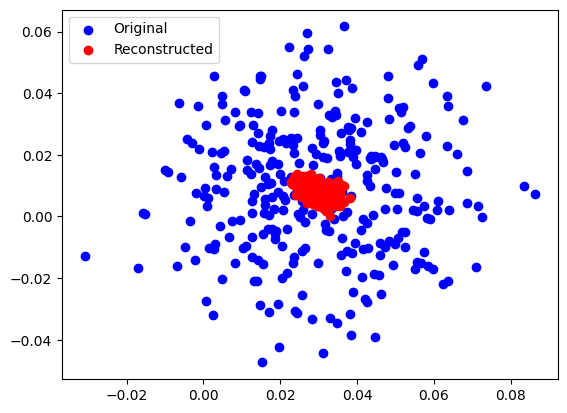
\includegraphics[width=0.4\textwidth]{figs/scatter2.png}
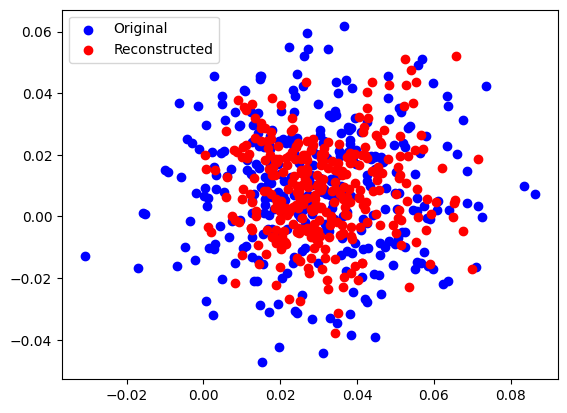
\includegraphics[width=0.4\textwidth]{figs/scatter1.png}
\caption{Left: Decoded Embeddings with MSE, Right: Decoded Embeddings with scaled MSE}
\end{figure}

The validation loss stops decreasing after 30 epochs for all configurations.
\begin{figure}[h!]
\centering
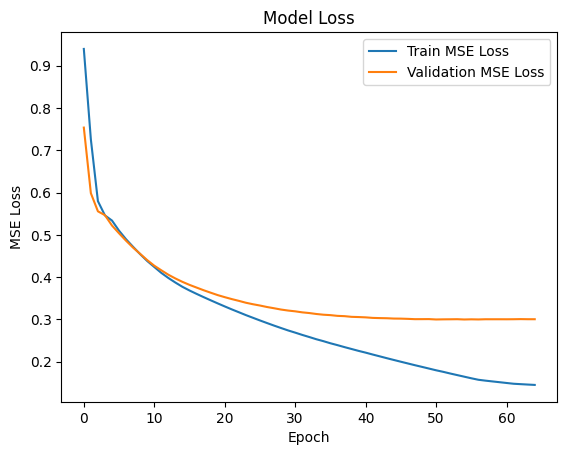
\includegraphics[width=0.4\textwidth]{figs/mse1-loss.png}
\caption{Loss plot for 768}
\end{figure}

We evaluate the performance of Autoencoder by first compare the clustering performance of the decoded embeddings with the original embeddings. We use KMeans clustering with 7 clusters and evaluate the performance using calinski-harabasz index, davis-bouldin index. 

\begin{center}
    
\begin{tabular}{|c|c|c|c|}
    \hline
    Model & DB score & CH score \\
    \hline
    KMeans on latent space(50) & 1.922802 & 29.529562 \\
    KMeans on original embeddings & 2.902679 & 13.327391 \\
    KMeans on UMAP embeddings(50) & 0.536476 & 454.550720 \\
    KMeans on UMAP embeddings(25) & 0.668492 & 352.116394 \\
    KMeans on UMAP embeddings(25) from latent space(50) & 0.719458 & 402.341339 \\
    \hline
\end{tabular}
\end{center}

The table above shows the clustering performance of the autoencoder and UMAP embeddings. We can see that the autoencoder is able to learn a some representation of the data and possibly reduce the noise if we compare the clustering performance of the decoded embeddings with the original embeddings. However, the performance of the autoencoder is not as good as the UMAP embeddings. The UMAP embeddings are able to capture the structure of the data and produce better clustering performance. We also tried to use the UMAP embeddings from the latent space of the autoencoder, but it does not improve the performance.

We then visualize the results of the autoencoder and UMAP embeddings using t-SNE. We use the same parameters for t-SNE as in our project. We set the perplexity to 20 and the number of iterations to 1000. We use the same color scheme as the original dataset. The t-SNE plot shows that the autoencoder is able to learn a compact representation of the data when compared to the original embeddings. However, the UMAP embeddings are able to capture the structure of the data better than the autoencoder. The UMAP embeddings are able to separate the clusters better and produce a more compact representation of the data.

\begin{figure}[h!]
\centering
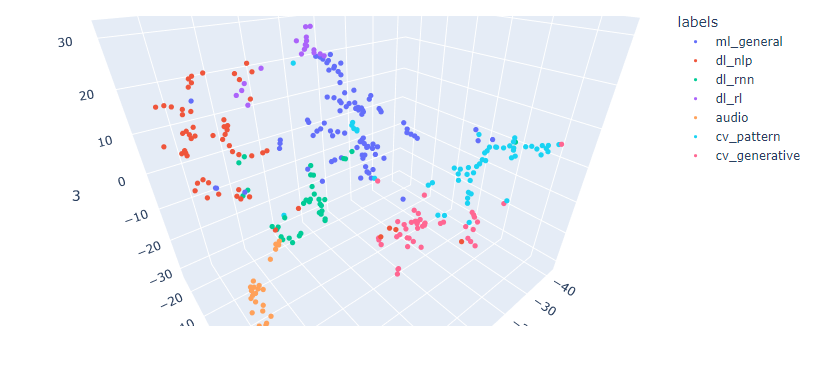
\includegraphics[width=0.8\textwidth]{figs/tsne1.png}
\caption{3D plot of original embeddings with t-SNE, labels are manually assigned based on the original dataset.}
\end{figure}

\begin{figure}[h!]
\centering
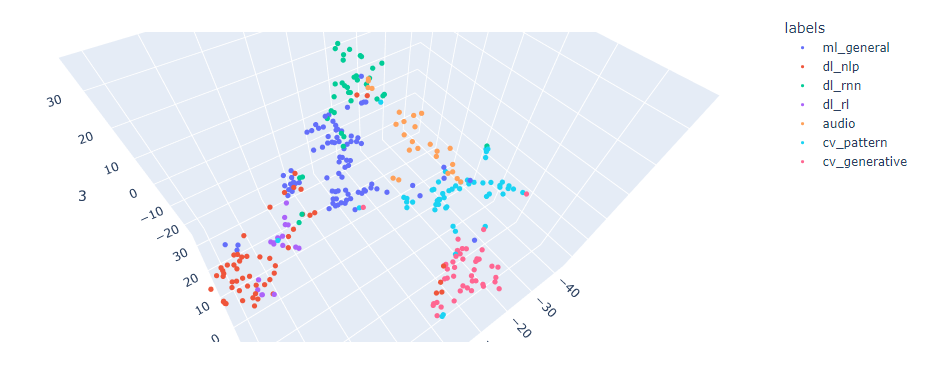
\includegraphics[width=0.8\textwidth]{figs/tsne2.png}
\caption{3D plot of decoded embeddings with t-SNE, labels are manually assigned based on the original dataset.}
\end{figure}

\begin{figure}[h!]
\centering
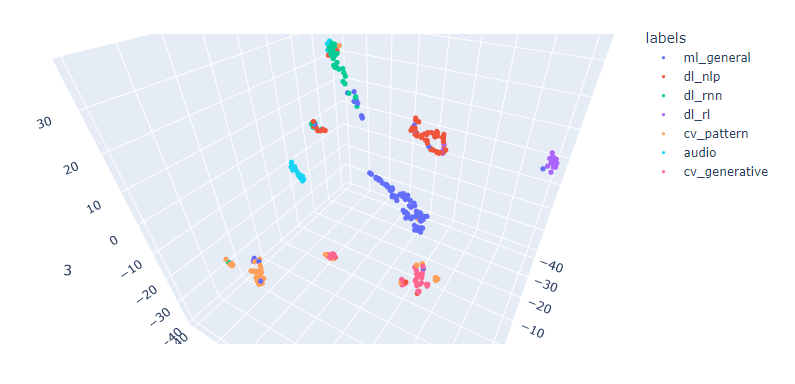
\includegraphics[width=0.8\textwidth]{figs/tsne3.png}
\caption{3D plot of umap-transformed embeddings with t-SNE, labels are manually assigned based on the original dataset.}
\end{figure}



\newpage
\section*{Gaussian Mixture Model and visualization}
We now move on to the dicussion of Gaussian Mixture Model. We apply the GMM to the latent space of the autoencoder. We use the same architecture as the autoencoder. We set the number of clusters to 10. We use the GMM with full covariance matrix. The reason we use 10 clusters instead of 7 is because we want to see if the GMM can capture the structure hiden during the merging operation.

To our surprise, the GMM is able to capture the structure of the data and produce better clustering on certain part of the data than what the tSNE plot shows. For example, in the tSNE plot, the two purple points at the bottom right are visually close to the blue points that are mostly computer vison paper. But a manual check shows that they should be classified as RNN papers. The GMM is able to capture this structure and produce a better clustering performance.

\begin{figure}[h!]
\centering
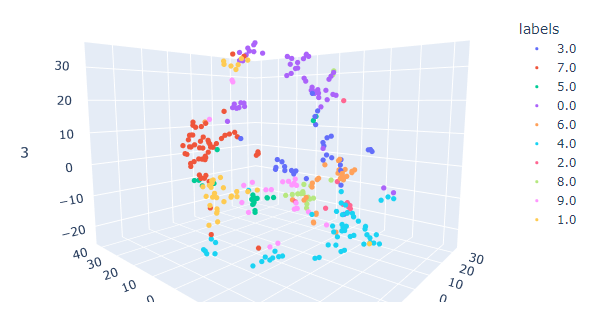
\includegraphics[width=0.8\textwidth]{figs/tsne4.png}
\caption{3D plot of GMM-clustered data with t-SNE, labels are automatically generated by the GMM.}
\end{figure}



\begin{table}
\centering
\begin{tabularx}{\textwidth}{lXX}
\toprule
Cluster & Paper1 & Paper2 \\
\midrule
0 & face recognition using eigenfaces & learning hierarchical features for scene labeling \\
1 & learning representations by back propagating errors & highly accurate protein structure prediction with alphafold \\
2 & context dependent pre trained deep neural networks for large vocabulary speech recognition & wavlm large scale self supervised pre training for full stack speech processing \\
3 & tensorf tensorial radiance fields & 3d gaussian splatting for real time radiance field rendering \\
4 & nearest neighbor pattern classification & no free lunch theorems for optimization \\
5 & hybrid computing using a neural network with dynamic external memory & photo real talking head with deep bidirectional lstm \\
6 & imagenet classification with deep convolutional neural networks & visual prompt tuning \\
7 & mathematical discoveries from program search with large language models funsearch & zero memory optimizations toward training trillion parameter models \\
8 & human level control through deep reinforcement learning & outracing champion gran turismo drivers with deep reinforcement learning sophy \\
9 & neural word embedding as implicit matrix factorization & self organized formation of topologically correct feature maps \\
\bottomrule
\end{tabularx}
\caption{Clusters and their representative papers}
\end{table}

The above table shows the clusters and 2 randomly sampled papers. The GMM successfully separated the representational theory,  classic machine learning papers, as well as the volumetric modeling papers which we didn't even considered as a group. And compare with agglomerative clustering  we used as the optimal cluster in the project, the GMM is not any inferior to that.

\section{Conclusion}

The combination of autoencoder and GMM is a good tool for clustering and dimensionality reduction. The autoencoder is able to learn a compact representation of the data and the GMM is able to capture the structure of the data. However, the performance of the autoencoder is not as good as the UMAP embeddings, possibly due to inadquate design of the neural network architecture. In the future, we can try to use a more complex architecture or a different loss function to improve the performance of the autoencoder. We can also try to use regularization techniques to prevent overfitting. 

The GMM is able to capture the structure of the data and produce better clustering on certain part of the data than what the tSNE plot shows. And to our surprise, the GMM is able to capture the structure of the data and produce better clustering on certain part of the data than what the tSNE plot shows and is it on par or even better than most of the clustering methods we used in the project. As a result, We should include GMM in our project as well.

\newpage
\bibliography{refs}
\bibliographystyle{plain}
\end{document}